\section{Results}\label{sec:results}

\subsection{Deterministic comparison}\label{sec:deterministic}

\sumpara On exact data the searched sequence beats EDD on all four instances, by the largest margins at 15 and 45 jobs. \sumparaend
\fin \Cref{tab:comparison} reports every method on every instance, and every one of these schedules is feasible. \fine
\fin Iterated greedy lowered total weighted tardiness relative to EDD by 17.1~percent on the 6-job instance, from 281 to 233 weighted minutes, and by 98.5, 97.6, and 81.0~percent on the development instances with 15, 45, and 120~jobs. \fine
\fin It also lowered total waiting on the three development instances, by 65.6, 61.1, and 61.8~percent, but raised it on the 6-job instance from 13 to 37~minutes. \fine
\fin \Cref{fig:comparison} shows both effects by instance size: the tardiness of the searched sequence is smallest relative to EDD at 15 and 45~jobs and rises to 19~percent of the EDD value at 120~jobs. \fine

\begin{table}[ht]
\centering
\caption{Deterministic comparison. Each row is one method on one instance, and every schedule is feasible. Seconds are the method's computation time on the laptop of \cref{sec:settings}. The optimum rows come from the mixed-integer program of \cref{sec:mip}; on the 15-job instance the optimal tardiness of 21 was reached by an order with 323~minutes of waiting.}
\label{tab:comparison}
\small
\begin{tabular}{llrrr}
\toprule
Instance (jobs) & Method & Total weighted tardiness & Total waiting & Seconds \\
\midrule
Hand-checkable (6) & Earliest due date & 281 & 13 & 0.000 \\
 & NEH\_EWDD only & 233 & 37 & 0.000 \\
 & Iterated greedy & 233 & 37 & 0.21 \\
 & Optimum (HiGHS) & 233 & 37 & 0.36 \\
\midrule
Small development (15) & Earliest due date & 1,417 & 732 & 0.000 \\
 & NEH\_EWDD only & 70 & 291 & 0.000 \\
 & Iterated greedy & 21 & 252 & 0.52 \\
 & Optimum (HiGHS) & 21 & 323 & 85.8 \\
\midrule
Medium development (45) & Earliest due date & 2,371 & 2,040 & 0.000 \\
 & NEH\_EWDD only & 360 & 1,068 & 0.000 \\
 & Iterated greedy & 58 & 794 & 3.22 \\
\midrule
Large development (120) & Earliest due date & 23,015 & 7,863 & 0.000 \\
 & NEH\_EWDD only & 9,452 & 3,928 & 0.003 \\
 & Iterated greedy & 4,383 & 3,005 & 37.2 \\
\bottomrule
\end{tabular}
\end{table}

\begin{figure}[ht]
\centering
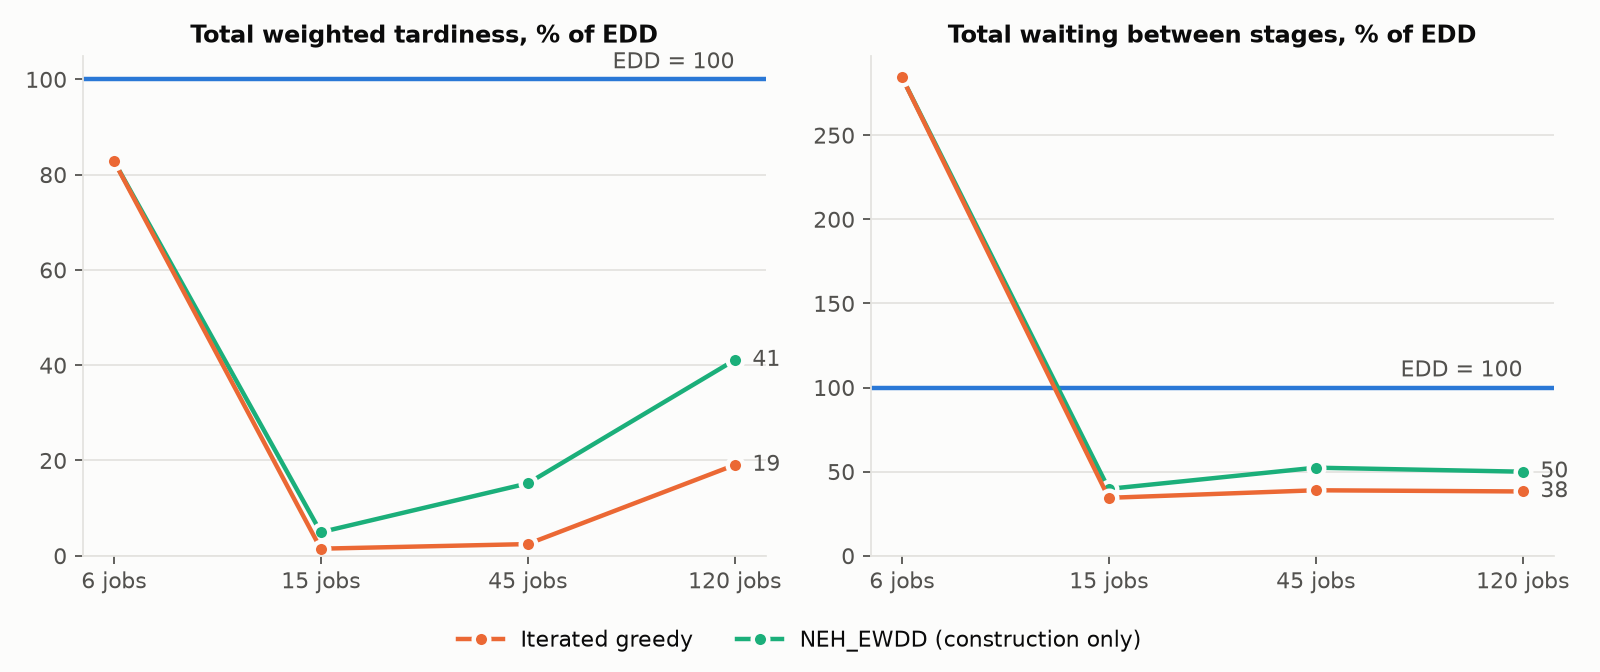
\includegraphics[width=\textwidth]{comparison/comparison.png}
\caption{Total weighted tardiness (left) and total waiting (right) of iterated greedy and of NEH\_EWDD alone, each as a percentage of the EDD value on the same instance (EDD is the line at 100). The horizontal axis gives the instance size; the labels at the right edge are the 120-job values. The two methods coincide on the 6-job instance.}
\label{fig:comparison}
\end{figure}

\sumpara The solver proves the searched values optimal where it can finish, and the seed matters only at 120 jobs. \sumparaend
\fin HiGHS proved the optimal total weighted tardiness to be 233 on the 6-job instance in 0.36~seconds and 21 on the 15-job instance in 85.8~seconds, and iterated greedy reached both values. \fine
\fin On the 15-job instance, the solver's optimal order had 323~minutes of waiting and iterated greedy's had 252, because only iterated greedy breaks ties in $Z$ by waiting. \fine
\fin With seeds 1 to 5, iterated greedy returned exactly the default seed's tardiness on the 6-, 15-, and 45-job instances, and values from 4,159 to 4,306 on the 120-job instance, all below the default seed's 4,383. \fine
\fin Its computation time grew from 0.21~seconds at 6~jobs to 37.2~seconds at 120~jobs, while EDD took under a millisecond on every instance. \fine

\subsection{Paired scenarios at a coefficient of variation of 0.2}\label{sec:stress-results}

\sumpara At a coefficient of variation of 0.2, the searched sequence stays far ahead of the EDD sequence on both measures in every scenario. \sumparaend
\fin \Cref{tab:stress} summarizes the two fixed sequences for the 45-job instance over the 30~saved scenarios at $\nu = 0.2$. \fine
\fin The iterated greedy sequence had the lower weighted tardiness in all 30~scenarios, with a mean of 420.6 weighted minutes against 3,541.1, a reduction of 3,120.5 weighted minutes (standard error 150.1 over the paired scenarios) or 88.1~percent, and a 90th percentile of 592.2 against 4,616.6. \fine
\fin In every scenario the reduction was at least 1,948.6 weighted minutes, and its 10th percentile was 2,235.1. \fine
\fin Its mean waiting was 1,276.9~minutes against 2,454.5, a reduction of 48.0~percent. \fine
\fin Neither sequence violated a hard constraint in any scenario, because right-shift execution preserves release dates, stage order, and one job per stage for any processing times, and due dates are soft targets. \fine
\fin \Cref{fig:stress} shows that the ranges do not overlap: the weighted tardiness of the iterated greedy sequence ranged from 103.3 to 1,120.0, and that of EDD from 2,276.2 to 6,013.8. \fine

\begin{table}[ht]
\centering
\caption{Stress test on the 45-job instance: 30~scenarios at a coefficient of variation of 0.2, seed 20261103. ``Planned'' is the value of the sequence on the exact data; the mean and the 90th percentile are over the scenarios. Tardiness is in weighted minutes and waiting in minutes.}
\label{tab:stress}
\small
\begin{tabular}{lrrrrrrr}
\toprule
 & \multicolumn{3}{c}{Total weighted tardiness} & \multicolumn{3}{c}{Total waiting} & Scenarios breaking \\
\cmidrule(lr){2-4}\cmidrule(lr){5-7}
Sequence & Planned & Mean & 90th pct. & Planned & Mean & 90th pct. & a hard constraint \\
\midrule
Earliest due date & 2,371.0 & 3,541.1 & 4,616.6 & 2,040.0 & 2,454.5 & 2,768.6 & 0 \\
Iterated greedy & 58.0 & 420.6 & 592.2 & 794.0 & 1,276.9 & 1,454.9 & 0 \\
\bottomrule
\end{tabular}
\end{table}

\begin{figure}[ht]
\centering
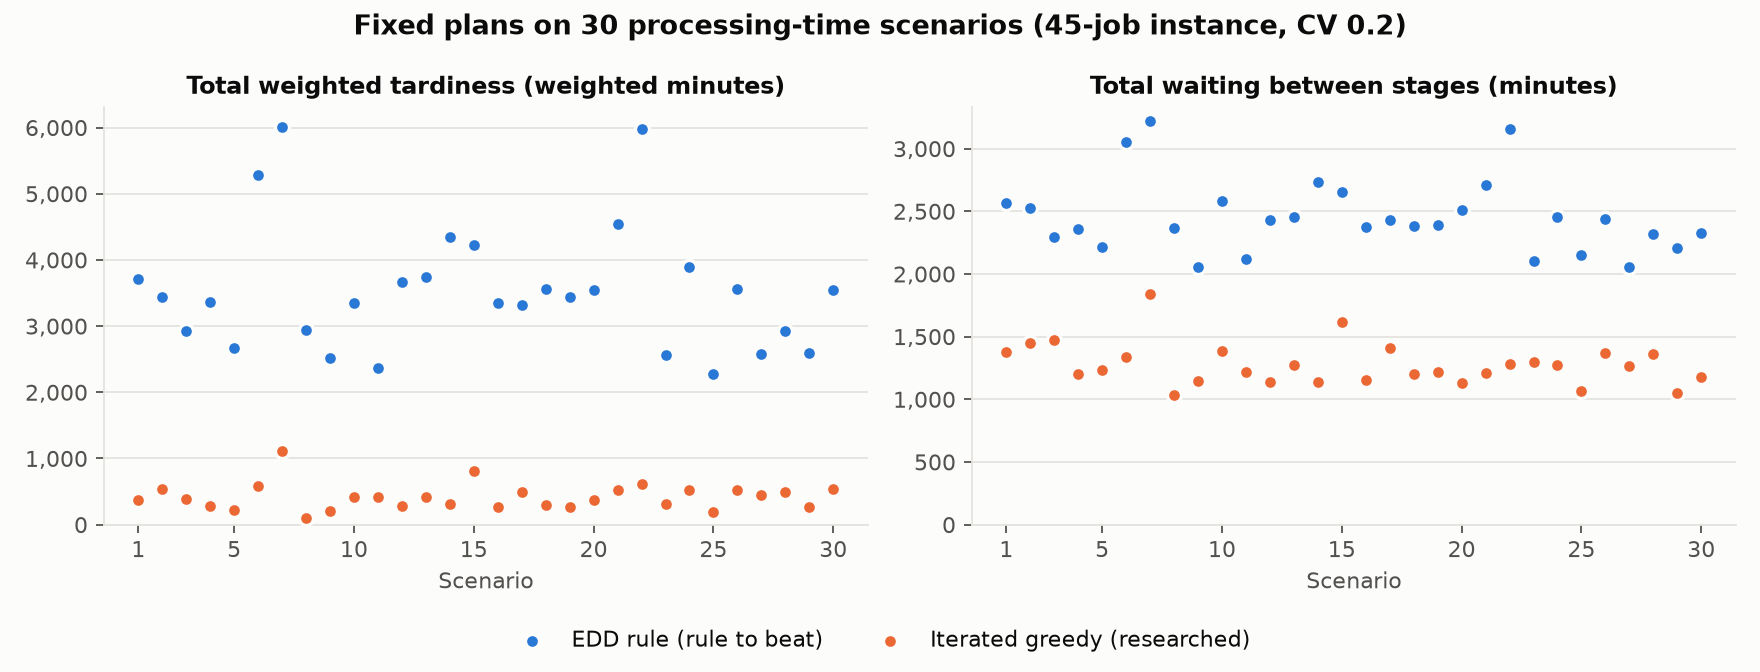
\includegraphics[width=\textwidth]{stress/stress_per_scenario.png}
\caption{Total weighted tardiness (left) and total waiting (right) of the two fixed sequences in each of the 30~scenarios of \cref{tab:stress}. Each dot is one sequence in one scenario, and both sequences face the same realized processing times in a scenario.}
\label{fig:stress}
\end{figure}

\subsection{Sensitivity to processing-time variability}\label{sec:sweep}

\sumpara Higher variability raises the tardiness of both sequences, cuts the relative advantage, and thins the worst periods' gain, while the mean gain holds. \sumparaend
\fin \Cref{tab:sweep} and \cref{fig:sweep} repeat the execution at five coefficients of variation, each with 30~new scenarios. \fine
\fin The mean weighted tardiness of the iterated greedy sequence rose from 148.1 at $\nu = 0.1$ to 8,901.6 at $\nu = 0.8$, and that of EDD from 2,720.1 to 12,230.5. \fine
\fin The relative reduction in mean weighted tardiness fell from 94.6~percent at $\nu = 0.1$ to 27.2~percent at $\nu = 0.8$. \fine
\fin The mean absolute reduction stayed between 2,572.0 and 3,683.7 weighted minutes at every level: it rose from $\nu = 0.1$ (standard error 65.9) to $\nu = 0.5$ (standard error 223.8), and its fall of 354.8 to 3,329.0 at $\nu = 0.8$ (standard error 342.7) is within the combined standard error of 409.3 of the two estimates. \fine
\fin The gain in a single period became less dependable at $\nu = 0.8$: the 10th percentile of the per-scenario reduction, between 1,781.1 and 2,473.2 weighted minutes at the lower levels, fell to 851.5, and the EDD sequence won 1 of the 30~scenarios, by 870.4 weighted minutes, its only win in the 180 paired scenarios of the six sets. \fine

\begin{table}[ht]
\centering
\caption{Sweep over variability on the 45-job instance. Each row uses 30~new scenarios, from seeds 6522 to 6526 in order. Tardiness is in weighted minutes. The reduction is the per-scenario difference between the two sequences' weighted tardiness: its mean, with the standard error in parentheses, and its 10th percentile; the percentage compares the two sequences' means.}
\label{tab:sweep}
\small
\setlength{\tabcolsep}{4.5pt}
\begin{tabular}{rrrrrrrr}
\toprule
 & \multicolumn{2}{c}{Earliest due date} & \multicolumn{2}{c}{Iterated greedy} & \multicolumn{3}{c}{Reduction} \\
\cmidrule(lr){2-3}\cmidrule(lr){4-5}\cmidrule(lr){6-8}
$\nu$ & Mean & 90th pct. & Mean & 90th pct. & Mean (s.e.) & 10th pct. & Percent \\
\midrule
0.1 & 2,720.1 & 3,171.6 & 148.1 & 228.4 & 2,572.0 (65.9) & 2,048.3 & 94.6 \\
0.2 & 3,273.5 & 4,425.0 & 407.2 & 643.9 & 2,866.4 (121.3) & 2,055.3 & 87.6 \\
0.3 & 4,139.8 & 6,213.4 & 952.5 & 1,676.0 & 3,187.3 (203.8) & 1,781.1 & 77.0 \\
0.5 & 6,680.4 & 9,498.8 & 2,996.7 & 5,434.2 & 3,683.7 (223.8) & 2,473.2 & 55.1 \\
0.8 & 12,230.5 & 17,420.0 & 8,901.6 & 14,219.8 & 3,329.0 (342.7) & 851.5 & 27.2 \\
\bottomrule
\end{tabular}
\end{table}

\begin{figure}[ht]
\centering
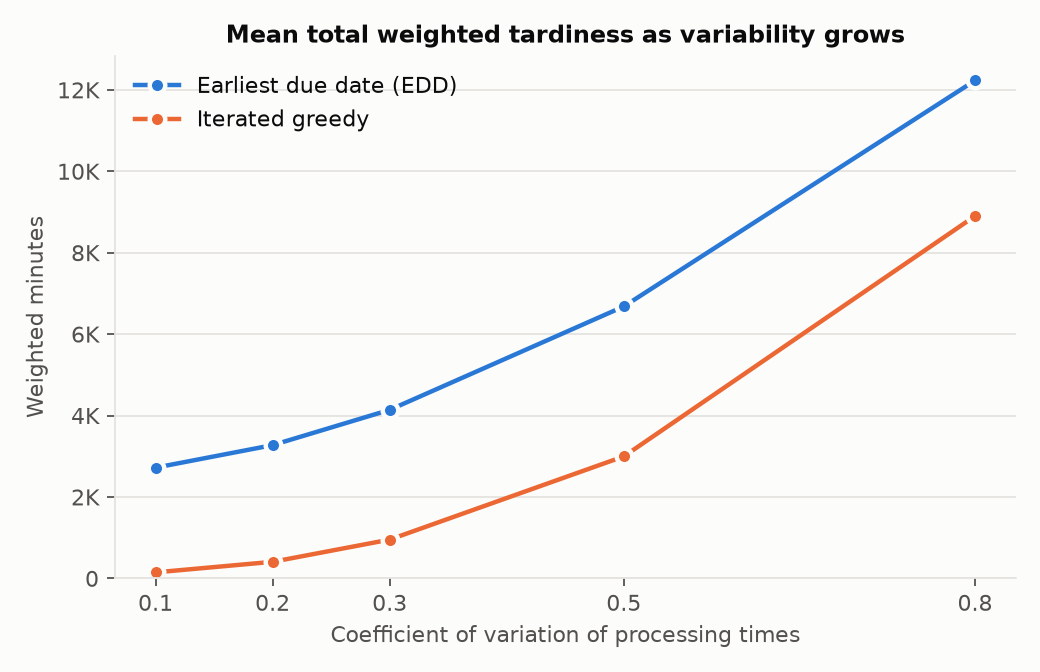
\includegraphics[width=0.62\textwidth]{stress/stress_cv_sweep.png}
\caption{Mean total weighted tardiness of the two fixed sequences for the 45-job instance at five coefficients of variation of the processing times, 30~scenarios each (\cref{tab:sweep}). The vertical gap between the lines is the absolute reduction, between 2,572.0 and 3,683.7 weighted minutes at every level.}
\label{fig:sweep}
\end{figure}
